\documentclass[letterpaper,doc]{apa6}

\usepackage{apacite}
\bibliographystyle{apacite}

\setkeys{Gin}{width=1\textwidth}

%%%%%%%%%%%%%%%%%%%%%%%%%%%%%%%%%%%%%%%%%%%%%%%%%%%%%%%%%%%%%%%%%%%%%%%%%%%%%%%
\title{Exploring the Relationship Between SAT Scores and First Year Retention}
\author{Jason Bryer}
\affiliation{Excelsior College}
\shorttitle{SAT and Retention}
%Optional components that can be added
%\journal{}
%\volume{}
%\ccoppy{Copyright notice}
%\copnum{Serial number or other reference}

%%%%%%%%%%%%%%%%%%%%%%%%%%%%%%%%%%%%%%%%%%%%%%%%%%%%%%%%%%%%%%%%%%%%%%%%%%%%%%%
\abstract{First year retention is an important measure for many institutions in determining whether first year college students return for a second year of college study. Many institutions rely on SAT scores as one indicator for determing college acceptance. This paper will utilize institional data from the Integrated Postsecondary Data System (IPEDS) to explore the relationship between SAT scores and first year retention rates.}


%%%%%%%%%%%%%%%%%%%%%%%%%%%%%%%%%%%%%%%%%%%%%%%%%%%%%%%%%%%%%%%%%%%%%%%%%%%%%%%
\usepackage{Sweave}
\begin{document}
\input{Retention-concordance}
\maketitle                            

The Integrated Postsecondary Education Data System (IPEDS) \citeA{ipeds} defines retention as:
\begin{quote}
A measure of the rate at which students persist in their educational program at an institution, expressed as a percentage. For four-year institutions , this is the percentage of first-time bachelors (or equivalent) degree-seeking undergraduates from the previous fall who are again enrolled in the current fall. For all other institutions this is the percentage of first-time degree/certificate-seeking students from the previous fall who either re-enrolled or successfully completed their program by the current fall.
\end{quote}

\section{Results}

% latex table generated in R 2.15.1 by xtable 1.7-0 package
% Fri Nov  2 14:56:59 2012
\begin{table}[ht]
\begin{center}
\begin{tabular}{rrrrr}
  \hline
 & Estimate & Std. Error & t value & Pr($>$$|$t$|$) \\ 
  \hline
(Intercept) & 63.0214 & 1.2954 & 48.65 & 0.0000 \\ 
  SATWriting & 0.0333 & 0.0092 & 3.61 & 0.0003 \\ 
  SATMath & 0.3435 & 0.0081 & 42.45 & 0.0000 \\ 
  AcceptanceTotal & -0.0354 & 0.0110 & -3.23 & 0.0013 \\ 
  UseAdmissionTestScoresRecommended & -7.0361 & 1.3721 & -5.13 & 0.0000 \\ 
  UseAdmissionTestScoresRequired & -6.8902 & 1.2375 & -5.57 & 0.0000 \\ 
   \hline
\end{tabular}
\caption{Regression Results}
\label{regressionTable}
\end{center}
\end{table}
\begin{figure}
\centering
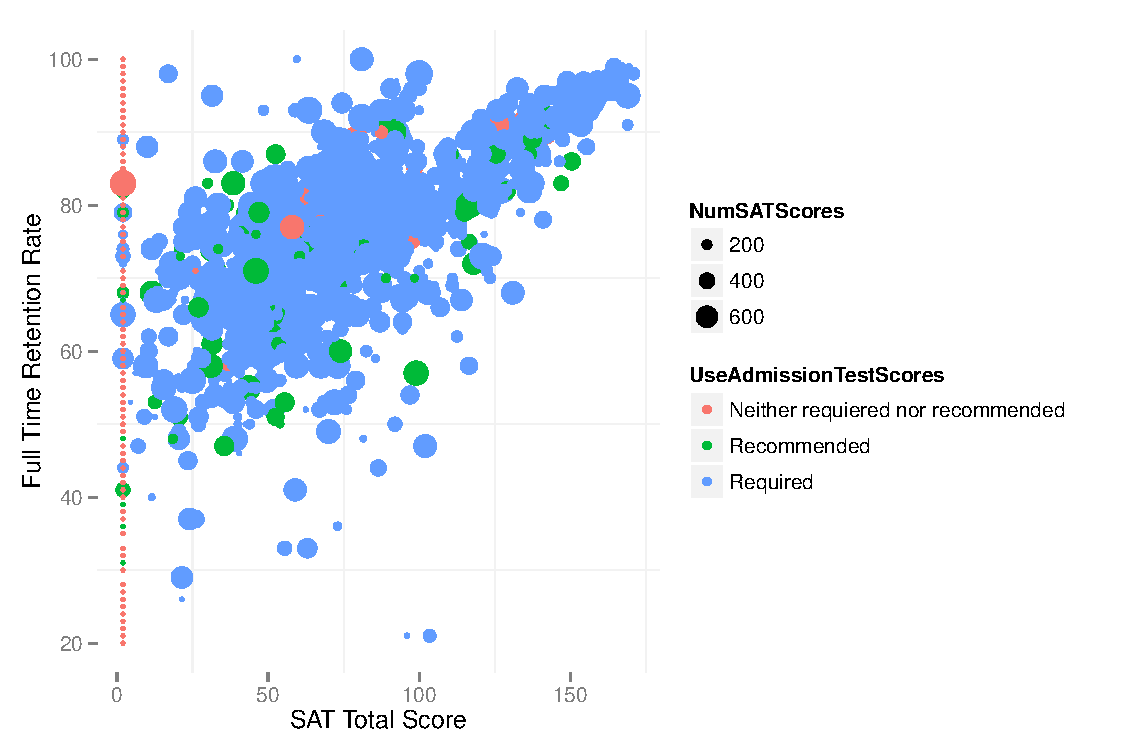
\includegraphics{Retention-003}
\caption{Relationship Between SAT Scores and Student Retention}
\label{fig:sat}
\end{figure}




%\clearpage

\bibliography{bibliography}

\end{document}

